% Generated by thesis/ch7/exp1/c4_units_figures.py -- do not edit by hand.
\begin{figure}[tbp]
  \centering
  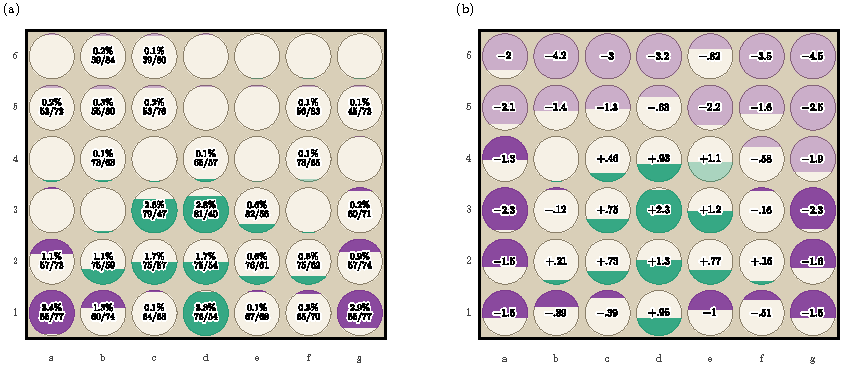
\includegraphics[width=\textwidth,height=0.8\textheight,keepaspectratio]{figures/ch7/c4-square-variance.pdf}
  \caption{Connect-4: which squares matter, in the outcome and to the network. (a) The outcome: share of the variance in who wins between the square's three states (x, empty, o); a full hole is 3.5\%; green filling from the bottom: holding the square helps its holder; purple from the top: it helps the other side; small numbers: x's chance of winning (\%) with x / with o on the square (shown with at least 30 positions each). (b) The network: the change in x's predicted log-odds from adding an x to the square, averaged over the training positions where it is empty; a full hole is 2.5; green from the bottom: good for x; purple from the top: bad for x. Pale, in both: filled in under 5\% of positions (in (b), values there are extrapolation).}
  \label{fig:ch7-c4-square-variance}
\end{figure}
